\documentclass[tikz]{standalone}

\usetikzlibrary{arrows.meta,fit,positioning}

\begin{document}
	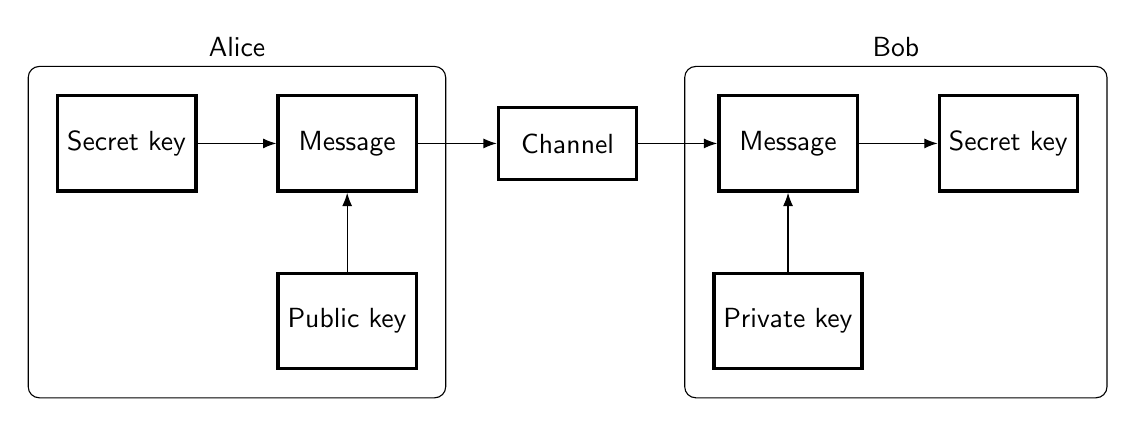
\begin{tikzpicture}[
		block/.style={draw, very thick, fill=white, minimum height=8ex, minimum width=5em},
		party/.style={draw, rounded corners, inner xsep=1em, inner ysep=1em},
		channel/.style={block, minimum height=6ex, minimum width=5em},
	]
		\node (ska) [block] {\textsf{Secret key}};
		\node (ma) [block, right=of ska] {\textsf{Message}};
		\node (pbk) [block, below=of ma] {\textsf{Public key}};
		\node (ch) [channel, right=of ma] {\textsf{Channel}};
		\node (mb) [block, right=of ch] {\textsf{Message}};
		\node (skb) [block, right=of mb] {\textsf{Secret key}};
		\node (prk) [block, below=of mb] {\textsf{Private key}};
		
		\node [party, label={\textsf{Alice}}, fit=(ska) (pbk)] {};
		\node [party, label={\textsf{Bob}}, fit=(skb) (prk)] {};
		
		\draw[-Latex] (ska) -- (ma);
		\draw[-Latex] (pbk) -- (ma);
		\draw[-Latex] (ma) -- (ch);
		\draw[-Latex] (ch) -- (mb);
		\draw[-Latex] (mb) -- (skb);
		\draw[-Latex] (prk) -- (mb);
	\end{tikzpicture}
\end{document}
